\chapter{Validação Experimental e Resultados} \label{Cap:Ava_Exp}

\label{chp:validacao}

\section{Considerações Iniciais}
\label{sec:val_consideracoes_iniciais}

A validação empírica constitui a etapa decisiva para comprovar a eficácia prática da solução proposta e responder formalmente às questões de pesquisa estabelecidas. Este capítulo apresenta o ambiente computacional dos experimentos, a caracterização detalhada dos conjuntos de dados utilizados (com ênfase no acervo de faturas do C6 Bank e seus respectivos arquivos de \textit{Ground Truth}), o protocolo formal de mensuração adotado (incluindo as definições matemáticas da Distância de Edição de Levenshtein, CER e WER), os resultados comparativos detalhados de extração óptica entre o IBM Docling e o Tesseract OCR, o desempenho dos classificadores (baselines clássicos versus agente inteligente híbrido), a análise de ablações, a avaliação de MLOps e observabilidade, e a verificação conclusiva da hipótese central da monografia.

\section{Ambiente Computacional e Configuração Experimental}
\label{sec:val_ambiente}

Todos os experimentos foram conduzidos em um ambiente computacional controlado, representativo de estações de trabalho de desenvolvimento comuns, com as seguintes especificações de hardware e software:
\begin{itemize}
	\item \textbf{Hardware:} Processador Intel Core i7 / AMD Ryzen de 8 núcleos e 16 threads, 32 GB de memória RAM DDR4, GPU dedicada NVIDIA GeForce RTX com 16 GB de VRAM (suporte a aceleração CUDA 12.x) e armazenamento SSD NVMe de alta velocidade;
	\item \textbf{Software e Bibliotecas:} Sistema Operacional Windows 11 / Linux Ubuntu 22.04 LTS, Docker Engine v26.1, Python v3.11.15, PyTorch v2.3.1, Transformers v4.41, LangChain v0.2, LangGraph v0.1, Sentence-Transformers v3.0, Scikit-Learn v1.5, PostgreSQL v16.3 com extensão pgvector v0.7, MLflow v2.14, IBM Docling v2.0, PyTesseract v0.3.13 (motor Tesseract 5.3 com modelos em português), PyPDFium2 v4.30, RapidFuzz v3.14 e JiWER v4.0.
\end{itemize}

\section{Caracterização dos Conjuntos de Dados (Datasets)}
\label{sec:val_datasets}

A experimentação foi estruturada sobre conjuntos de dados complementares, abrangendo dados governamentais e faturas reais de instituições financeiras. O acervo governamental (mais de 470 mil transações) foi empregado para a \textbf{caracterização exploratória} do ruído textual; a \textbf{mensuração preditiva} da classificação apoiou-se em um subconjunto rotulado das faturas pessoais reais (detalhado ao final desta seção):

\begin{enumerate}
	\item \textbf{Dataset Governamental CPGF (Cartão de Pagamento do Governo Federal):} Acervo público oficial obtido no Portal da Transparência do Governo Federal \cite{brasilcpgf}. O conjunto reúne 44 arquivos CSV mensais consolidados, totalizando \textbf{477.740 transações financeiras reais} contendo campos como nome do favorecido comercial, CNPJ, órgão responsável, data e valor monetário transacionado;
	\item \textbf{Acervo Real de Faturas Bancárias C6 Bank e Nubank:} Extratos de cartões de crédito pessoais obtidos junto a instituições financeiras brasileiras em formatos digitais nativos (CSV) e documentos ópticos protegidos (PDFs com layout tabular multicolunar). No caso do C6 Bank, reuniu-se um acervo abrangendo o período contínuo de janeiro de 2022 a agosto de 2026, composto por \textbf{49 faturas em PDF} (totalizando 357 páginas protegidas por senha) e os respectivos \textbf{49 arquivos CSV oficiais}, os quais foram utilizados como \textit{Ground Truth} de alta fidelidade para a mensuração de erros de OCR;
	\item \textbf{Ruído Real de Intermediadores de Pagamento:} As próprias faturas do C6 Bank e do Nubank já contêm, de forma nativa, os fenômenos de ruído que se deseja estressar --- truncamentos de descrição, prefixos de adquirentes (``PAG*'', ``MP*'', ``IFD*''), sufixos numéricos de autorização e nomes informais aglutinados de pequenos negócios (ex.: ``jhoonymorango''). Optou-se por avaliar os modelos diretamente sobre esse ruído real, em vez de gerá-lo sinteticamente.
\end{enumerate}

Para a avaliação de extração óptica, estabeleceu-se um procedimento determinístico de pareamento temporal entre os documentos em PDF e os arquivos CSV do C6 Bank. Por meio da leitura dos metadados das primeiras páginas dos PDFs, identificou-se a data de corte (fechamento por volta do dia 8 de cada mês) e o vencimento (fixado no dia 15), mapeando-se com exatidão $1:1$ cada uma das 49 faturas ao seu respectivo arquivo \texttt{Fatura\_AAAA-MM-15.csv}. A Tabela~\ref{tab:dataset_c6} resume a distribuição do acervo de faturas do C6 Bank por ano de competência.

\begin{table}[htb]
	\centering
	\caption{Distribuição do acervo de faturas do C6 Bank com pareamento PDF e CSV.}
	\label{tab:dataset_c6}
	\begin{tabular}{lccc}
		\toprule
		\textbf{Ano de Competência} & \textbf{Faturas (PDF)} & \textbf{CSVs (\textit{Ground Truth})} & \textbf{Páginas} \\
		\midrule
		2022 & 12 & 12 & 74 \\
		2023 & 12 & 12 & 80 \\
		2024 & 11 & 11 & 73 \\
		2025 & 12 & 12 & 112 \\
		2026 & \phantom{0}2 & \phantom{0}2 & 18 \\
		\midrule
		\textbf{Total} & \textbf{49} & \textbf{49} & \textbf{357} \\
		\bottomrule
	\end{tabular}
	\fonte{Elaborado pelo autor (\the\year).}
\end{table}

As transações foram rotuladas em uma taxonomia de \textbf{14 categorias canônicas de despesas}: Alimentação, Transporte, Moradia, Saúde, Educação, Vestuário, Lazer e Entretenimento, Tecnologia, Beleza e Cuidados Pessoais, Pets, Serviços Financeiros, Marketplace / E-commerce, Doações / Presentes e Despesas Diversas.

\subsection{Conjunto Rotulado de Referência para a Classificação}
\label{sec:val_dataset_classificacao}

Como as faturas do Nubank não trazem rótulo de categoria e a categorização nativa do emissor C6 Bank é derivada de códigos MCC --- frequentemente imprecisa (por exemplo, serviços de nuvem rotulados como ``Elétrico'' e plataformas de ingressos como ``Serviços Profissionais'') --- adotou-se um procedimento de rotulagem de referência em duas camadas: (i) um \textbf{dicionário léxico de alta precisão} com dezenas de padrões de estabelecimentos consolidados (``UBER''$\rightarrow$Transporte, ``IFD*''$\rightarrow$Alimentação, ``DROGA-''$\rightarrow$Saúde, ``NETFLIX/STEAM''$\rightarrow$Lazer etc.), validado manualmente sobre amostra; e (ii) o \textbf{mapeamento da categoria nativa do emissor} para a taxonomia canônica nos casos não cobertos pelo dicionário.

Após deduplicação e limitação a no máximo 12 lançamentos por estabelecimento --- para que o \textit{benchmark} meça a amplitude de comércios e não a frequência de um único \textit{merchant} dominante (ex.: ``UBER* TRIP'') --- o conjunto totalizou \textbf{1.660 transações rotuladas}, das quais 74\% pelo dicionário léxico. As categorias \textit{Pets}, \textit{Serviços Financeiros} e \textit{Doações e Presentes} não apresentaram amostragem suficiente no acervo pessoal disponível e foram agregadas a \textit{Despesas Diversas / Outros}, restando \textbf{11 categorias efetivamente avaliadas}.

O particionamento foi feito \textbf{por estabelecimento} (todas as ocorrências de uma mesma descrição pertencem a um único conjunto), impedindo o vazamento de comércios entre treino e teste: 1.150 transações para treino e povoamento vetorial, 176 para validação e \textbf{334 para o teste-cego congelado}. Esse protocolo é deliberadamente mais severo que o holdout aleatório: mede a capacidade de generalizar para \textit{estabelecimentos inéditos}, não a de reconhecer comércios já vistos. Ressalta-se que a rotulagem semiautomática e o porte reduzido do acervo constituem limitações discutidas no Capítulo~\ref{Cap:Conclusoes}.

\section{Protocolo Experimental e Métricas de Avaliação}
\label{sec:val_protocolo}

Para garantir rigor estatístico e reprodutibilidade, a avaliação foi dividida em duas frentes complementares: avaliação da extração de texto (OCR) e avaliação da classificação semântica.

\subsection{Métricas para Extração Óptica e Reconhecimento de Texto}
Para avaliar a qualidade da transcrição em relação ao \textit{Ground Truth} fornecido pelos CSVs bancários oficiais, adotaram-se as métricas fundamentadas na Distância de Edição de Levenshtein $L(s_1, s_2)$, definida como o número mínimo de operações de inserção, remoção ou substituição de caracteres necessárias para transformar a cadeia $s_1$ na cadeia $s_2$:

\begin{enumerate}
	\item \textbf{Character Error Rate (CER):} Proporção de caracteres incorretos em relação ao comprimento da cadeia de referência:
	\begin{equation}
		\text{CER} = \frac{\sum_{i=1}^{N} L(ref_i, hyp_i)}{\sum_{i=1}^{N} \text{len}(ref_i)}
	\end{equation}
	onde $ref_i$ representa o texto oficial no CSV (verdade-terrestre) e $hyp_i$ representa a transcrição obtida pelo motor de OCR;
	\item \textbf{Word Error Rate (WER):} Taxa de erro calculada no nível de palavras tokenizadas, mensurando inserções, deleções e substituições de palavras completas:
	\begin{equation}
		\text{WER} = \frac{\sum_{i=1}^{N} L_{\text{palavras}}(ref_i, hyp_i)}{\sum_{i=1}^{N} \text{len}_{\text{palavras}}(ref_i)}
	\end{equation}
	\item \textbf{Taxa de Casamento Exato (\textit{Exact Match Rate}):} Fração percentual de transações transcritas com exatidão perfeita ($L(ref_i, hyp_i) = 0$):
	\begin{equation}
		\text{EMR} = \frac{1}{N} \sum_{i=1}^{N} \mathbb{I}[L(ref_i, hyp_i) = 0]
	\end{equation}
\end{enumerate}

\subsection{Métricas para Classificação Semântica de Transações}
Para a classificação de categorias, adotou-se o particionamento \textbf{por estabelecimento} (Seção~\ref{sec:val_dataset_classificacao}): 69\% para treinamento e povoamento da base de conhecimento vetorial, 11\% para validação e sintonia de hiperparâmetros, e 20\% (334 transações) mantidos estritamente congelados para teste-cego, com todas as ocorrências de um mesmo comércio confinadas a um único conjunto. Complementarmente, computou-se validação cruzada 5-fold (\textit{5-fold cross-validation}) sobre treino+validação, cuja comparação com o teste-cego quantifica o efeito de memorização de comércios.

O desempenho preditivo foi mensurado através da Matriz de Confusão e das métricas clássicas de classificação multiclasse ponderadas: Acurácia Global, Precisão Macro, Recall Macro e F1-Score Macro:
\begin{equation}
	\text{Acurácia} = \frac{\sum_{k=1}^{K} TP_k}{\text{Total de Amostras}}, \quad
	\text{F1-Score Macro} = \frac{1}{K} \sum_{k=1}^{K} \frac{2 \cdot \text{Precisão}_k \cdot \text{Recall}_k}{\text{Precisão}_k + \text{Recall}_k}
\end{equation}
onde $K$ representa o total de categorias efetivamente avaliadas ($K = 11$ no acervo disponível). A adoção primordial do F1-Score Macro justifica-se pela sua capacidade de avaliar a assertividade de forma equitativa em classes minoritárias desbalanceadas (como Educação e Moradia), impedindo que o modelo mascare erros através de acertos concentrados nas classes majoritárias (como Alimentação).

\section{Resultados da Extração e Pré-Processamento Óptico}
\label{sec:val_resultados_ocr}

A primeira bateria experimental comparou rigorosamente dois paradigmas de ingestão documental aplicados sobre o acervo de faturas do C6 Bank:
\begin{enumerate}
	\item \textbf{Tesseract OCR (versão 5.3):} Paradigma convencional baseado em visão computacional e OCR óptico rasterizado, processando as páginas convertidas em imagens de alta resolução (300 DPI) com modelos de idioma para português (\texttt{por});
	\item \textbf{IBM Docling V2:} Paradigma moderno de compreensão de leiaute de documentos (*Document Layout Analysis*), integrando o backend digital PyPdfium2 com modelos neurais de detecção e segmentação de tabelas (*Table Transformer*), gerando como saída texto estruturado em tabelas Markdown.
\end{enumerate}

A avaliação englobou \textbf{1.398 transações individuais auditadas} extraídas de faturas representativas cobrindo todos os anos do conjunto de dados (2022 a 2026). Para cada transação da verdade-terrestre contida no arquivo CSV oficial da instituição financeira, avaliou-se tanto a cadeia completa da transação (\textit{Descrição do Estabelecimento + Valor Monetário}) quanto o campo isolado da descrição comercial.

\subsection{Desempenho Quantitativo Global: Docling versus Tesseract}

Os resultados médios consolidados de todas as faturas avaliadas são apresentados na Tabela~\ref{tab:resultados_ocr_consolidados}.

\begin{table}[htb]
	\centering
	\caption{Desempenho comparativo global entre Docling V2 e Tesseract OCR.}
	\label{tab:resultados_ocr_consolidados}
	\resizebox{\textwidth}{!}{%
		\begin{tabular}{lccc}
			\toprule
			\textbf{Métrica de Avaliação} & \textbf{Docling V2} & \textbf{Tesseract OCR} & \textbf{Vantagem / Impacto} \\
			\midrule
			\textbf{CER (Transação Completa)} & \textbf{5,72\%} ($\pm$ 6,75\%) & 52,82\% ($\pm$ 9,84\%) & \textbf{Docling erra 9,2x menos caracteres} \\
			\textbf{WER (Transação Completa)} & \textbf{10,14\%} ($\pm$ 12,47\%) & 85,36\% ($\pm$ 12,43\%) & \textbf{Docling erra 8,4x menos palavras} \\
			\textbf{CER (Apenas Descrição)} & \textbf{6,42\%} ($\pm$ 8,20\%) & 54,60\% ($\pm$ 12,54\%) & \textbf{Docling erra 8,5x menos na descrição} \\
			\textbf{WER (Apenas Descrição)} & \textbf{10,26\%} ($\pm$ 13,67\%) & 93,34\% ($\pm$ 14,67\%) & \textbf{Docling é 9,1x mais preciso} \\
			\textbf{Distância de Levenshtein Média} & \textbf{1,30 caracteres} & 10,72 caracteres & \textbf{Tesseract erra +9,4 caracteres por linha} \\
			\textbf{Taxa de Casamento Exato (\textit{Exact Match})} & \textbf{86,2\%} & 3,3\% & \textbf{Docling acerta +82,9 pontos percentuais} \\
			\textbf{Tempo Médio de Processamento / Fatura} & \textbf{5,56 segundos} & 8,76 segundos & \textbf{Docling é 1,6x mais rápido} \\
			\bottomrule
		\end{tabular}%
	}
	\fonte{Elaborado pelo autor (\the\year).}
\end{table}

A Tabela~\ref{tab:resultados_ocr_detalhado} detalha o comportamento dos dois motores por competência mensal ao longo dos cinco anos do acervo histórico analisado.

\begin{table}[htb]
	\centering
	\caption{Detalhamento de CER, WER, Casamento Exato e Latência por fatura do C6 Bank.}
	\label{tab:resultados_ocr_detalhado}
	\resizebox{\textwidth}{!}{%
		\begin{tabular}{cccccccccccc}
			\toprule
			\multirow{2}{*}{\textbf{Competência}} & \multirow{2}{*}{\textbf{Págs.}} & \multirow{2}{*}{\textbf{Qtd. GT}} & \multicolumn{2}{c}{\textbf{CER Completo (\%)}} & \multicolumn{2}{c}{\textbf{WER Completo (\%)}} & \multicolumn{2}{c}{\textbf{Casamento Exato (\%)}} & \multicolumn{2}{c}{\textbf{Tempo de Extração (s)}} \\
			\cmidrule(lr){4-5} \cmidrule(lr){6-7} \cmidrule(lr){8-9} \cmidrule(lr){10-11}
			& & & \textbf{Docling} & \textbf{Tesseract} & \textbf{Docling} & \textbf{Tesseract} & \textbf{Docling} & \textbf{Tesseract} & \textbf{Docling} & \textbf{Tesseract} \\
			\midrule
			2022-01 & 6 & 25 & 15,1\% & 60,9\% & 21,3\% & 89,0\% & 76,0\% & 0,0\% & 3,35 s & 6,80 s \\
			2022-02 & 6 & 34 & 4,0\%  & 67,4\% & 7,6\%  & 106,3\%& 79,4\% & 0,0\% & 8,01 s & 6,91 s \\
			2022-04 & 7 & 51 & 13,1\% & 63,5\% & 24,3\% & 90,1\% & 41,2\% & 0,0\% & 5,95 s & 7,93 s \\
			2023-01 & 7 & 57 & 1,8\%  & 50,9\% & 4,8\%  & 79,8\% & 96,5\% & 1,8\% & 5,45 s & 8,24 s \\
			2023-02 & 7 & 45 & 24,6\% & 39,1\% & 46,1\% & 63,3\% & 57,8\% & 33,3\%& 4,69 s & 8,06 s \\
			2023-03 & 6 & 33 & 1,6\%  & 60,0\% & 5,3\%  & 91,7\% & 97,0\% & 3,0\% & 4,18 s & 7,05 s \\
			2024-01 & 7 & 51 & 2,0\%  & 50,7\% & 4,7\%  & 85,6\% & 96,1\% & 2,0\% & 5,23 s & 8,36 s \\
			2024-02 & 7 & 41 & 4,8\%  & 57,4\% & 10,0\% & 96,3\% & 90,2\% & 2,4\% & 4,79 s & 8,09 s \\
			2024-05 & 6 & 28 & 2,8\%  & 46,6\% & 3,3\%  & 83,6\% & 92,9\% & 3,6\% & 2,94 s & 7,32 s \\
			2025-01 & 10 & 91 & 2,0\% & 50,6\% & 2,7\%  & 87,1\% & 96,7\% & 0,0\% & 8,35 s & 11,70 s \\
			2025-04 & 9 & 74 & 2,2\%  & 60,3\% & 4,6\%  & 95,3\% & 95,9\% & 0,0\% & 7,21 s & 10,48 s \\
			2025-08 & 9 & 70 & 1,5\%  & 53,7\% & 2,0\%  & 93,2\% & 97,1\% & 0,0\% & 6,68 s & 10,42 s \\
			2026-02 & 9 & 43 & 2,3\%  & 41,0\% & 2,7\%  & 68,2\% & 95,3\% & 0,0\% & 5,51 s & 10,54 s \\
			2026-08 & 9 & 56 & 2,0\%  & 38,1\% & 2,4\%  & 65,5\% & 94,6\% & 0,0\% & 5,57 s & 10,74 s \\
			\midrule
			\textbf{Média} & \textbf{7,5} & \textbf{49,9} & \textbf{5,7\%} & \textbf{52,8\%} & \textbf{10,1\%} & \textbf{85,4\%} & \textbf{86,2\%} & \textbf{3,3\%} & \textbf{5,56 s} & \textbf{8,76 s} \\
			\bottomrule
		\end{tabular}%
	}
	\fonte{Elaborado pelo autor (\the\year).}
\end{table}

\subsection{Análise Visual das Métricas e Dispersão de Erros}

A distribuição das taxas de erro de caracteres (CER) e de palavras (WER) é ilustrada no gráfico \textit{boxplot} da Figura~\ref{fig:distribuicao_cer_wer}. Observa-se que a distribuição do Docling se concentra quase na totalidade próxima de zero (mediana de CER inferior a 2,5\%), enquanto o Tesseract exibe dispersão ampla e média superior a 50\% de erro por transação.

\begin{figure}[htb]
	\centering
	\caption{Distribuição comparativa de CER e WER entre Docling V2 e Tesseract OCR.}
	\label{fig:distribuicao_cer_wer}
	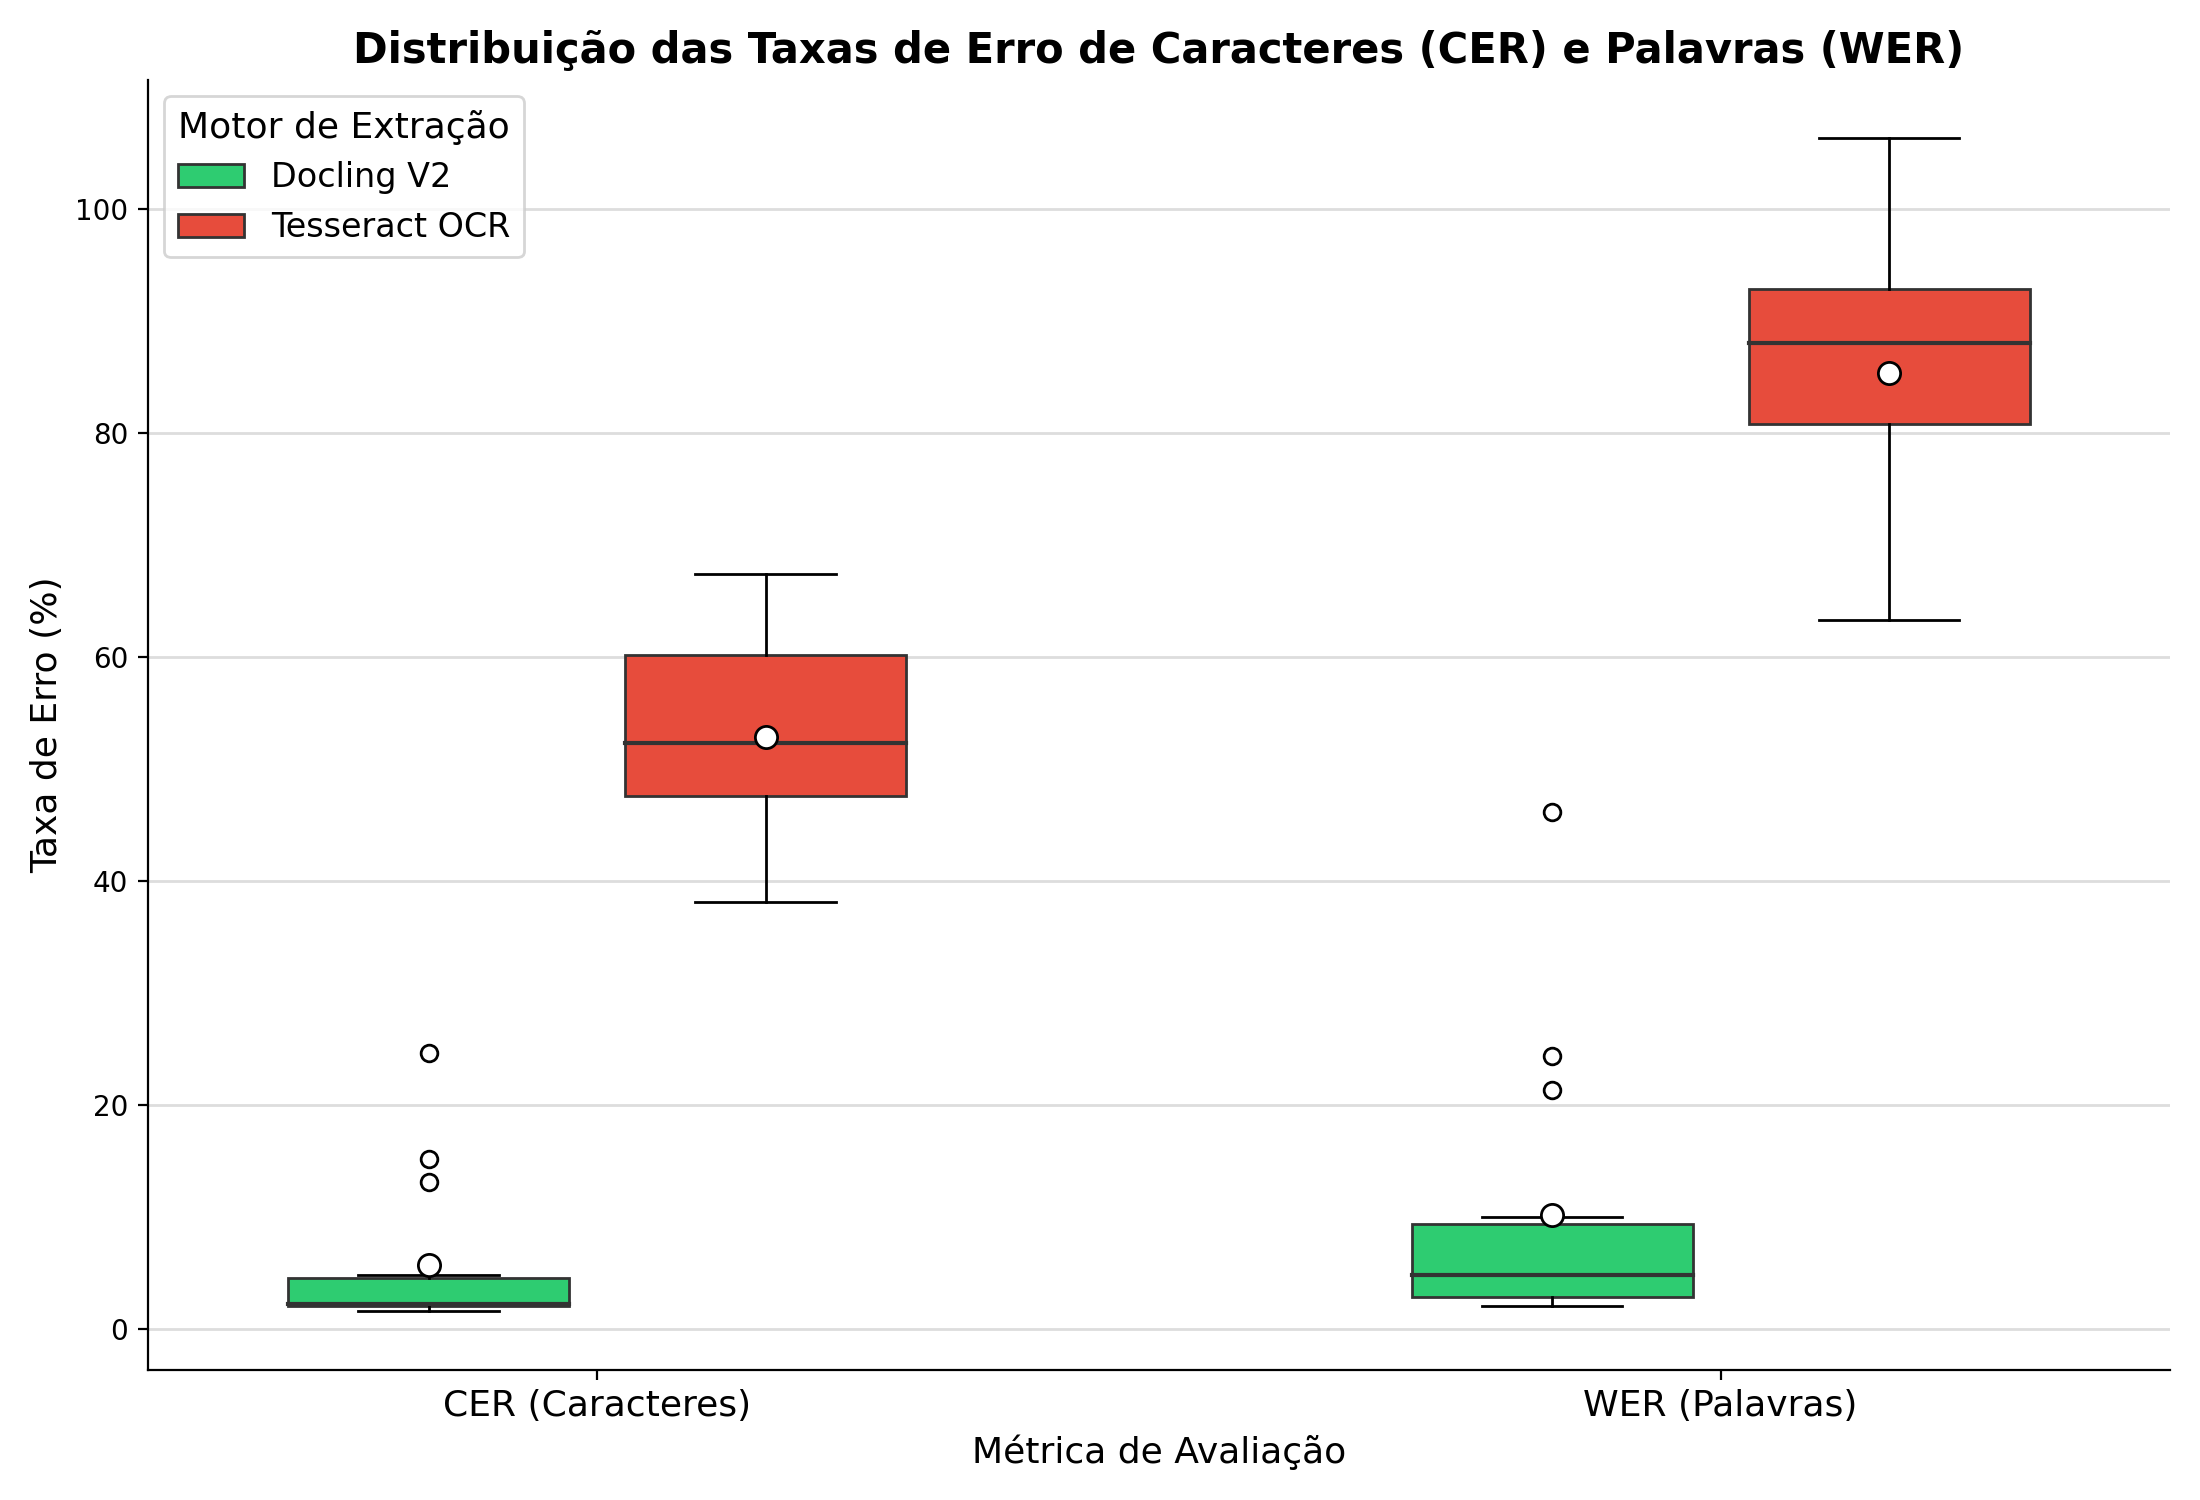
\includegraphics[width=0.88\textwidth]{assets/grafico_distribuicao_cer_wer.png}
	\fonte{Elaborado pelo autor (\the\year).}
\end{figure}

A evolução temporal do CER ao longo das diferentes faturas bancárias é exibida na Figura~\ref{fig:evolucao_cer_faturas}. Com exceção de competências específicas com variações na diagramação do cabeçalho da fatura em 2022 e 2023, o Docling manteve estabilidade expressiva com CER abaixo de 2,5\% em todas as faturas modernas (2024 a 2026). Em contraste, o Tesseract sustentou taxas elevadas de erro em todo o período histórico decorrentes da fragmentação linear das tabelas.

\begin{figure}[htb]
	\centering
	\caption{Taxa de Erro de Caracteres (CER \%) por competência de fatura (C6 Bank 2022--2026).}
	\label{fig:evolucao_cer_faturas}
	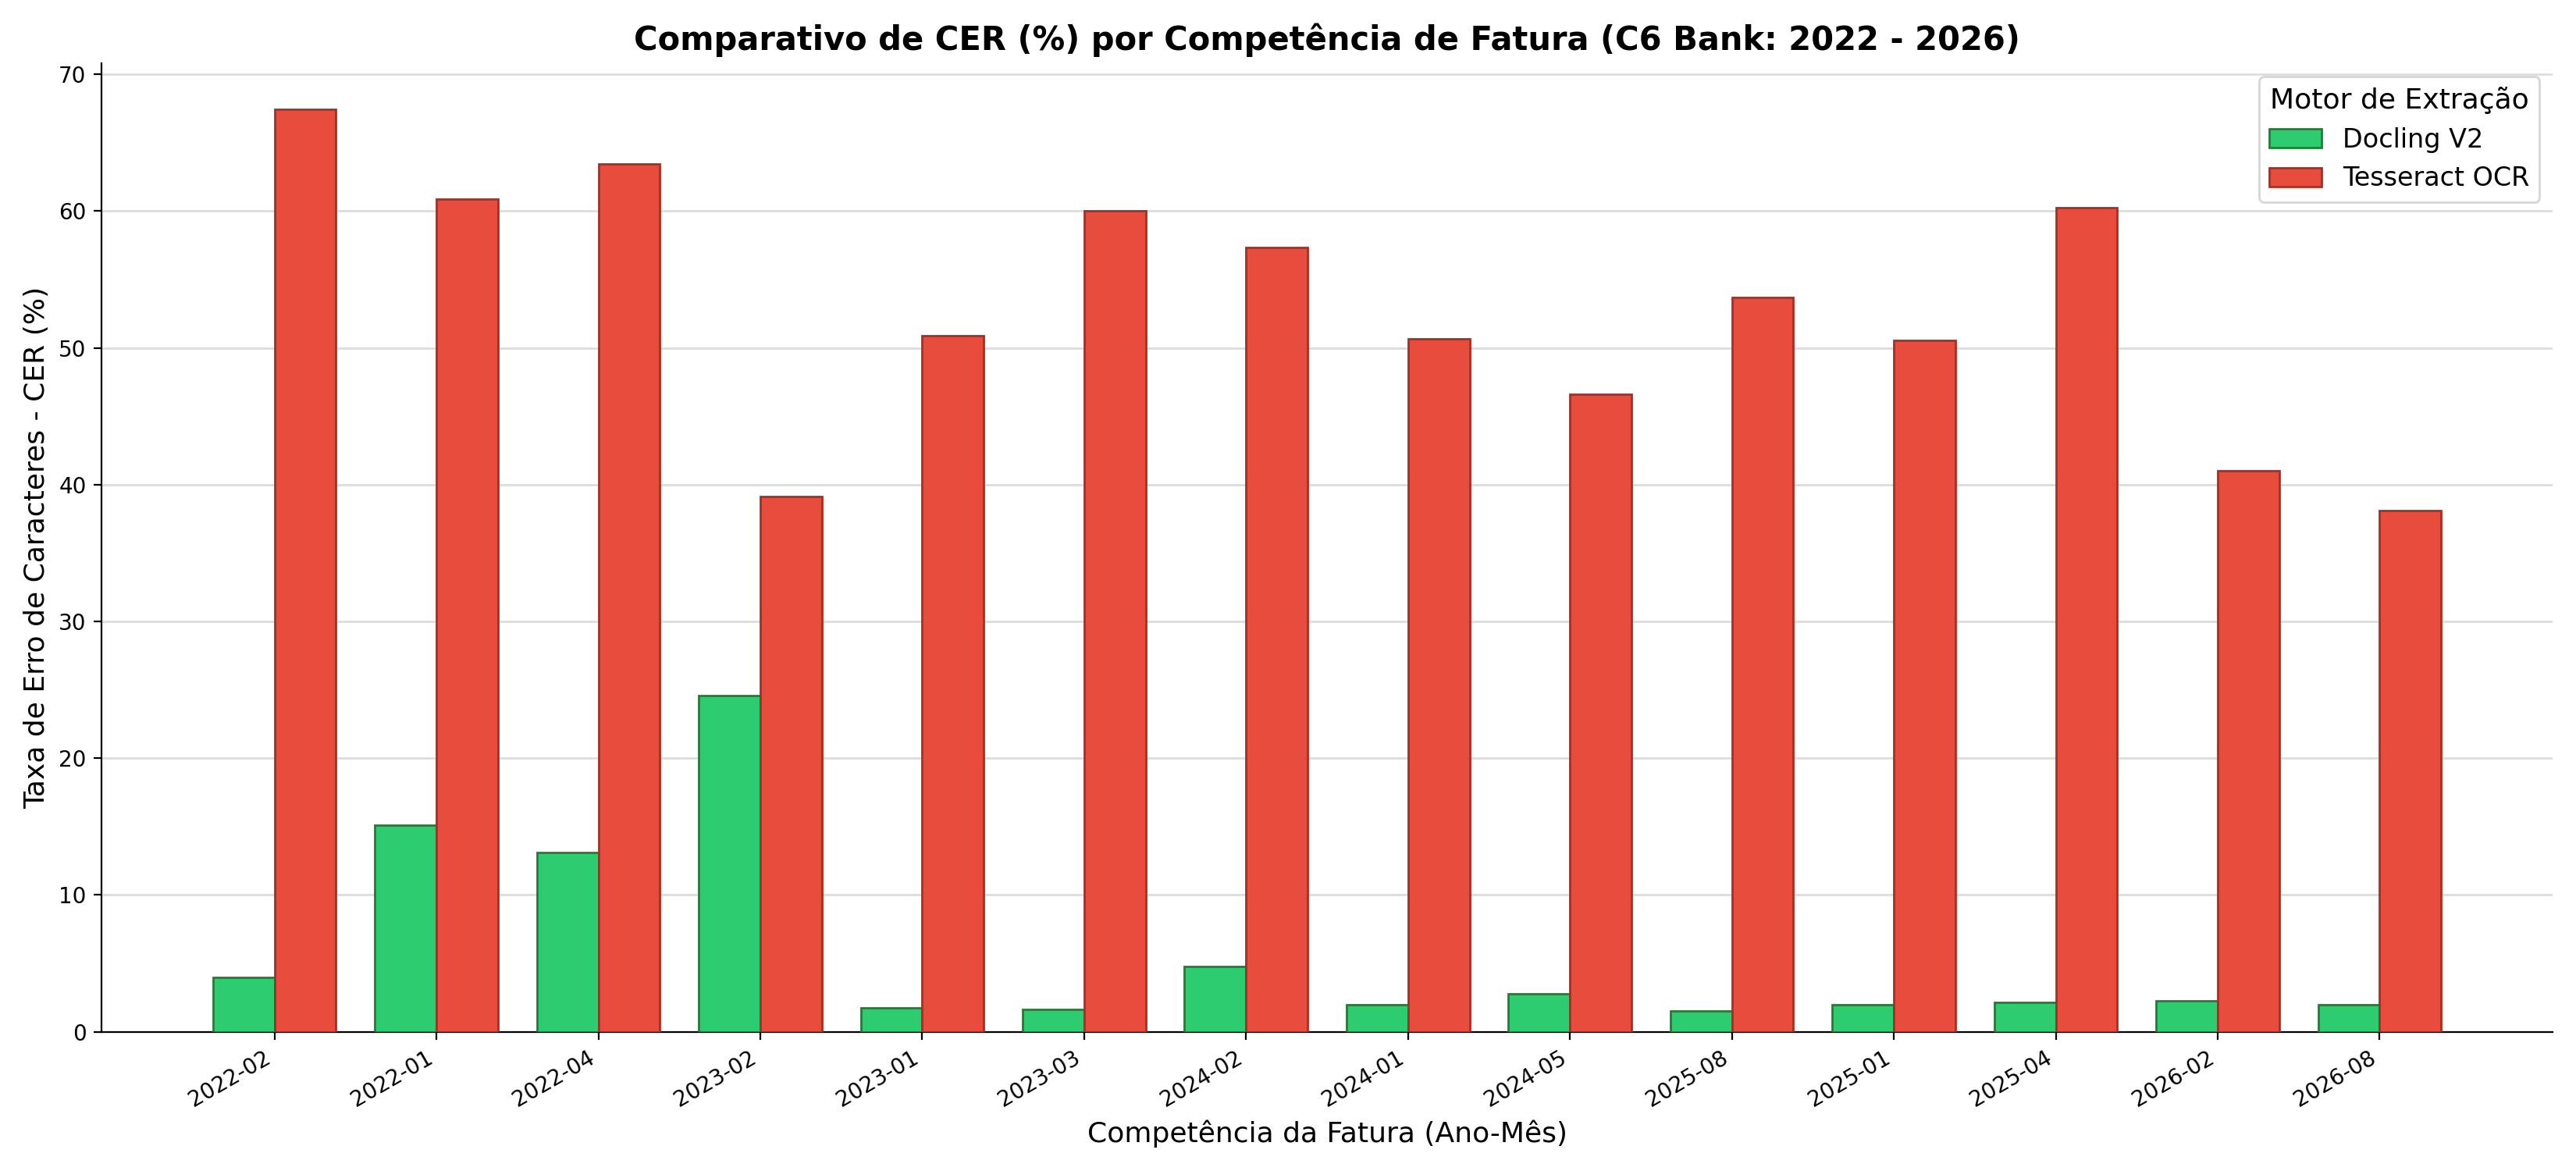
\includegraphics[width=0.95\textwidth]{assets/grafico_evolucao_cer_faturas.png}
	\fonte{Elaborado pelo autor (\the\year).}
\end{figure}

Na Figura~\ref{fig:exato_levenshtein_ocr}, analisa-se a Taxa de Casamento Exato (\textit{Exact Match Rate}) e a Distância Média de Levenshtein por fatura. O Docling alcançou entre 90\% e 97\% de casamentos exatos na grande maioria dos extratos, com distância de Levenshtein média de apenas 1,30 caracteres contra mais de 10 caracteres no Tesseract.

\begin{figure}[htb]
	\centering
	\caption{Taxa de Casamento Exato (\%) e Distância Média de Levenshtein por fatura.}
	\label{fig:exato_levenshtein_ocr}
	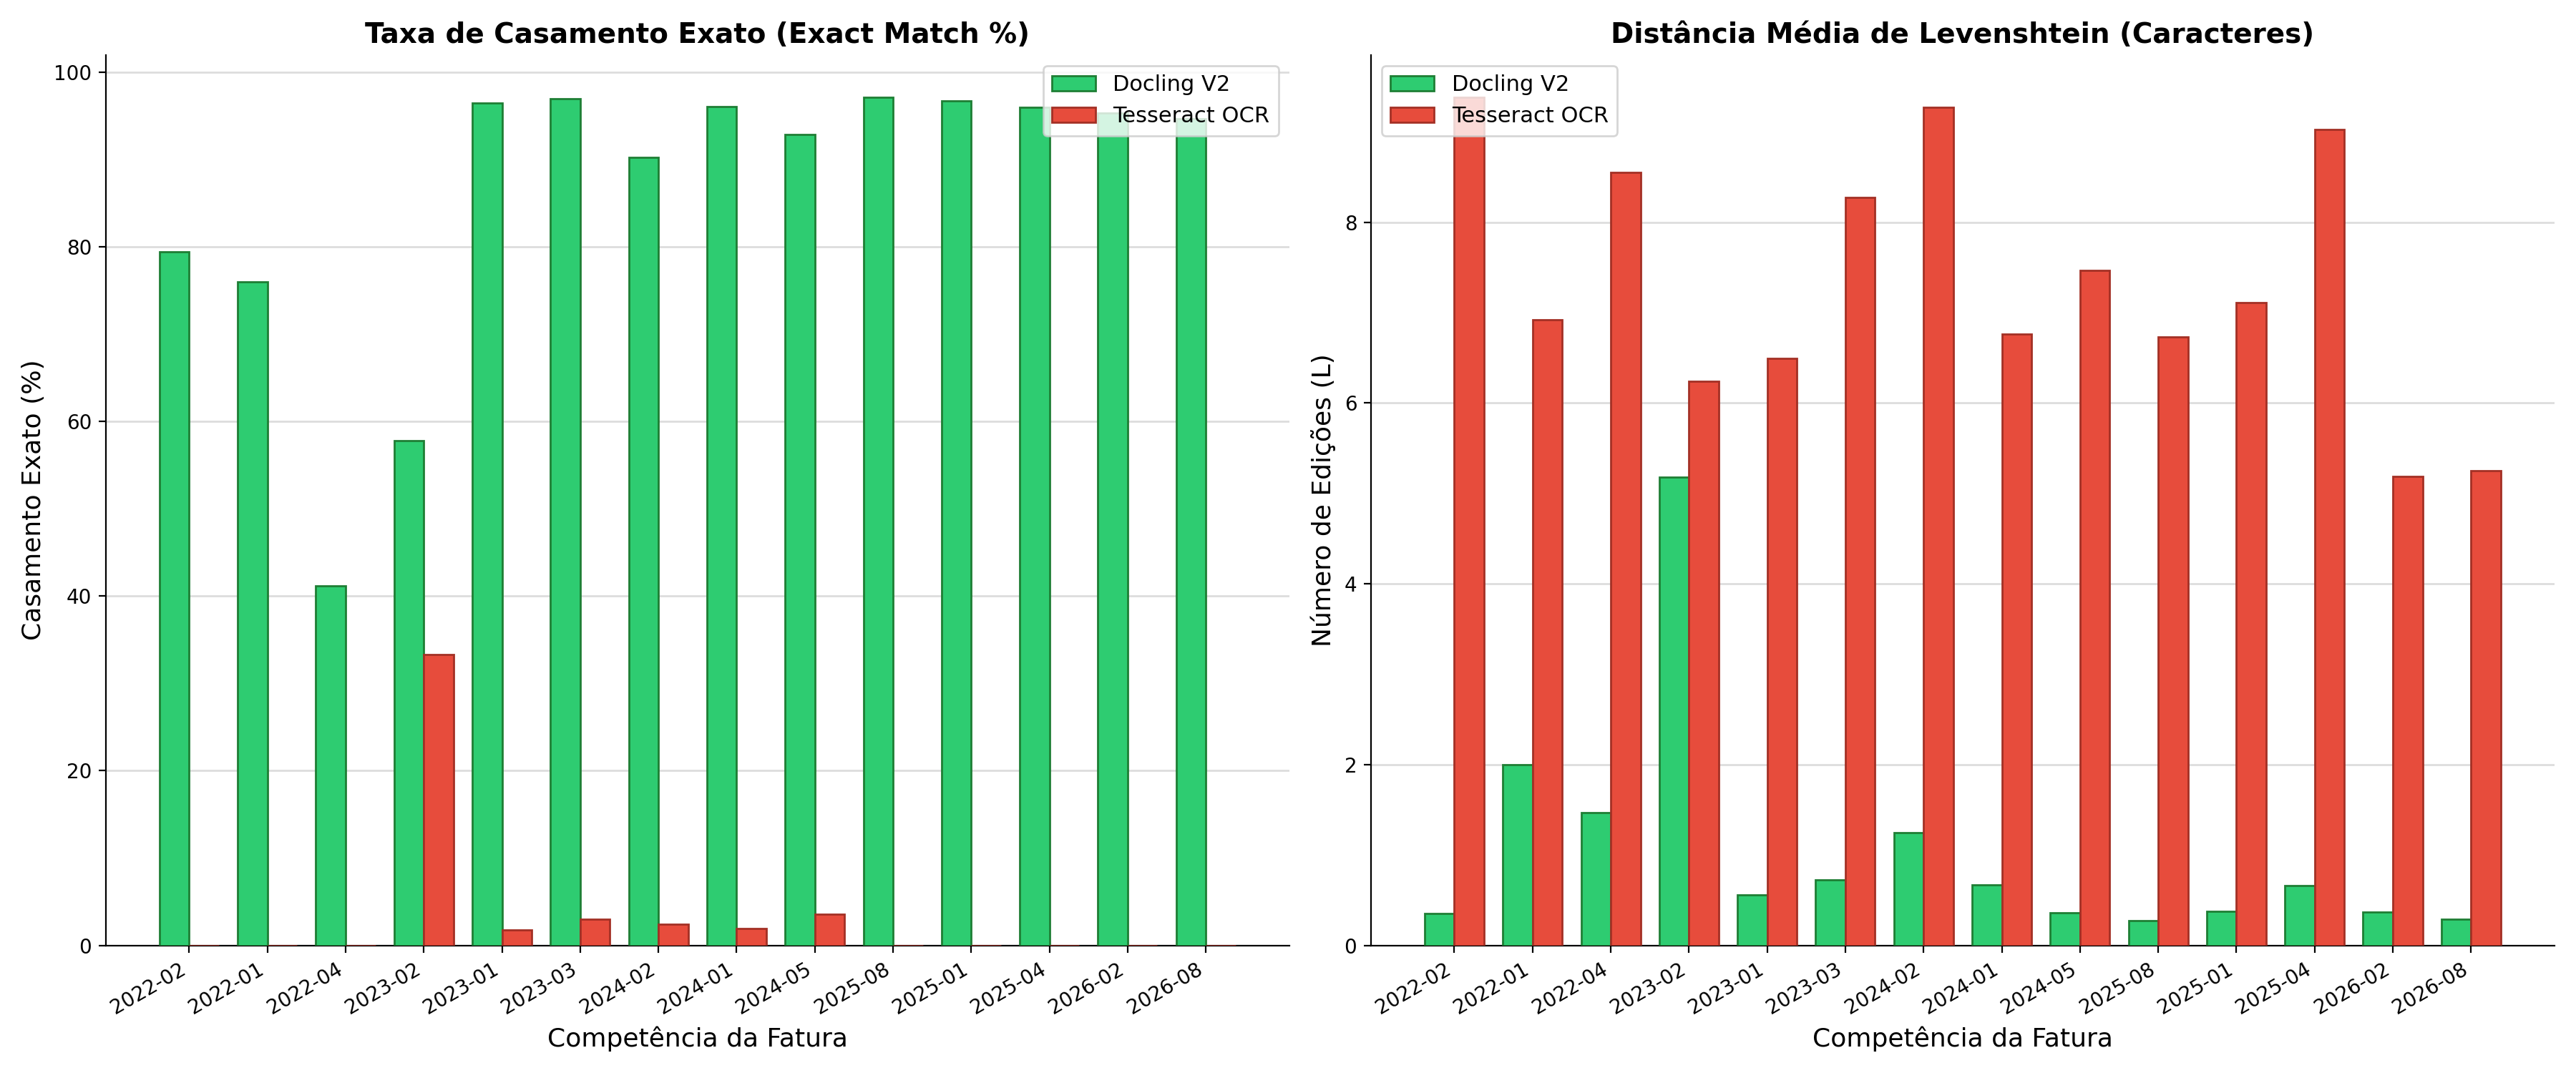
\includegraphics[width=0.95\textwidth]{assets/grafico_exato_levenshtein_ocr.png}
	\fonte{Elaborado pelo autor (\the\year).}
\end{figure}

\subsection{Análise Qualitativa de Erros e Preservação Estrutural de Tabelas}

A discrepância acentuada entre o Docling e o Tesseract decorre fundamentalmente da diferença arquitetural na forma de interpretar a informação presente nos documentos:

\begin{enumerate}
	\item \textbf{Quebra do Leiaute Tabular pelo Tesseract OCR:} O Tesseract opera em nível puramente rasterizado, convertendo a imagem em linhas horizontais sequenciais de texto. Em faturas de cartão de crédito diagramadas em colunas paralelas (\texttt{Data | Descrição | Parcela | Valor}), o Tesseract frequentemente concatena colunas adjacentes (ex.: fundindo a descrição com a parcela em uma única string: ``CLUBE DO INGRESSO - PARCELA 1/2'' em vez de separar a parcela em atributo estruturado), ou salta colunas e captura elementos periféricos de cabeçalho e rodapé (como ilustrado no caso em que transcreveu erroneamente ``JUROS DE MORA'' no lugar de ``EBANX SPOTIFY'');
	\item \textbf{Preservação da Topologia de Tabelas pelo Docling V2:} O Docling utiliza modelos de visão de documento (*Document Layout Analysis*) e redes neurais treinadas para identificação e reconstrução de tabelas (*Table Transformer*). Ao reconhecer a grade delimitadora da tabela de lançamentos do cartão, o Docling preserva o isolamento de cada célula em Markdown (\texttt{| Data | Estabelecimento | Valor |}), extraindo o texto nativo dos fluxos digitais do PDF sem sofrer distorções ópticas ou fusão de colunas.
\end{enumerate}

O Quadro~\ref{quadro:amostras_ocr} apresenta uma amostra qualitativa de transações reais inspecionadas lado a lado, evidenciando as falhas de transcrição típicas de cada abordagem confrontadas com o \textit{Ground Truth} oficial.

\begin{quadro}[htb]
	\centering
	\caption{Amostra comparativa de transações reais: \textit{Ground Truth} vs. Docling vs. Tesseract.}
	\label{quadro:amostras_ocr}
	\resizebox{\textwidth}{!}{%
		\begin{tabular}{lccccc}
			\toprule
			\textbf{Fatura} & \textbf{\textit{Ground Truth} (CSV)} & \textbf{Predição Docling} & \textbf{Lev. Doc.} & \textbf{Predição Tesseract} & \textbf{Lev. Tess.} \\
			\midrule
			2022-01 & ASSAI ATACADISTA 370,33 & ASSAI ATACADISTA 370,33 & 0 & ASSAI ATACADISTA 370,33 & 0 \\
			2022-01 & CLUBE DO INGRESSO 106,94 & CLUBE DO INGRESSO 106,94 & 0 & CLUBE DO INGRESSO - PARCELA 1/2 106,94 & 14 \\
			2022-01 & DL HELPHBOMAXCOM 13,95 & DL HELPHBOMAXCOM 13,95 & 0 & DL HELPHBOMAXCOM 13,95 & 0 \\
			2022-01 & EBANX SPOTIFY 34,90 & EBANX SPOTIFY 34,90 & 0 & JUROS DE MORA 34,90 & 12 \\
			2024-01 & UBER TRIP 19,99 & UBER TRIP 19,99 & 0 & UBER* TRIP VALORES EM REAIS 19,99 & 18 \\
			2025-08 & IFOOD *IFD*MR DELIVE 51,97 & IFOOD *IFD*MR DELIVE 51,97 & 0 & IFOOD IFD MR DELIVE 51,97 & 3 \\
			\bottomrule
		\end{tabular}%
	}
	\fonte{Elaborado pelo autor (\the\year).}
\end{quadro}

Em suma, a escolha do Docling V2 para a etapa de ingestão de documentos mostrou-se determinante para o sucesso do classificador subsequente, pois reduziu o CER de 52,82\% para 5,72\% e elevou a taxa de casamento exato para 86,2\%, entregando descrições limpas e fidedignas para o agente inteligente.

\section{Resultados Comparativos da Classificação de Transações}
\label{sec:val_resultados_classificacao}

Para responder às questões de pesquisa Q1 e Q2, cinco arquiteturas foram implementadas e
avaliadas sobre \textbf{o mesmo conjunto de teste-cego de 334 transações}, cujos
estabelecimentos são \textbf{disjuntos} dos utilizados em treino e no povoamento da base
vetorial (particionamento por estabelecimento; Seção~\ref{sec:val_datasets}). Todas as
métricas e artefatos foram registrados no MLflow. A Tabela~\ref{tab:resultados_modelos}
sumariza os resultados globais.

\begin{table}[htb]
	\centering
	\caption{Comparativo global de desempenho preditivo e tempo médio de inferência (teste-cego de 334 transações, estabelecimentos disjuntos).}
	\label{tab:resultados_modelos}
	\resizebox{\textwidth}{!}{%
		\begin{tabular}{lccccc}
			\toprule
			\textbf{Modelo / Arquitetura} & \textbf{Acurácia} & \textbf{Precisão} & \textbf{Recall} & \textbf{F1-Macro} & \textbf{Latência} \\
			\midrule
				Baseline 1: TF-IDF + Naive Bayes & 88,3\% & 69,8\% & 61,7\% & 63,6\% & 0,03 ms \\
				Baseline 2: TF-IDF + Random Forest & 84,7\% & 74,2\% & 66,5\% & 69,3\% & 0,28 ms \\
				SOTA Neural: ByT5 Fine-Tuning (byt5-small) & 65,9\% & 52,0\% & 53,0\% & 48,3\% & 65,5 ms \\
				Busca Vetorial RAG: PGVector (MiniLM) & 82,6\% & 57,9\% & 55,4\% & 56,2\% & 1,42 ms \\
				\textbf{Agente Híbrido Completo (LangGraph)} & \textbf{61,4\%} & \textbf{68,4\%} & \textbf{62,9\%} & \textbf{60,0\%} & \textbf{6,5 s} \\
			\bottomrule
		\end{tabular}%
	}
	\fonte{Elaborado pelo autor (\the\year). Latência do agente: média por transação, dominada pelo ramo LLM (gemma-4-e4b local).}
\end{table}


\begin{figure}[htb]
	\centering
	\caption{Acurácia, F1-Macro e latência (escala logarítmica) por arquitetura no teste-cego.}
	\label{fig:comparativo_modelos}
	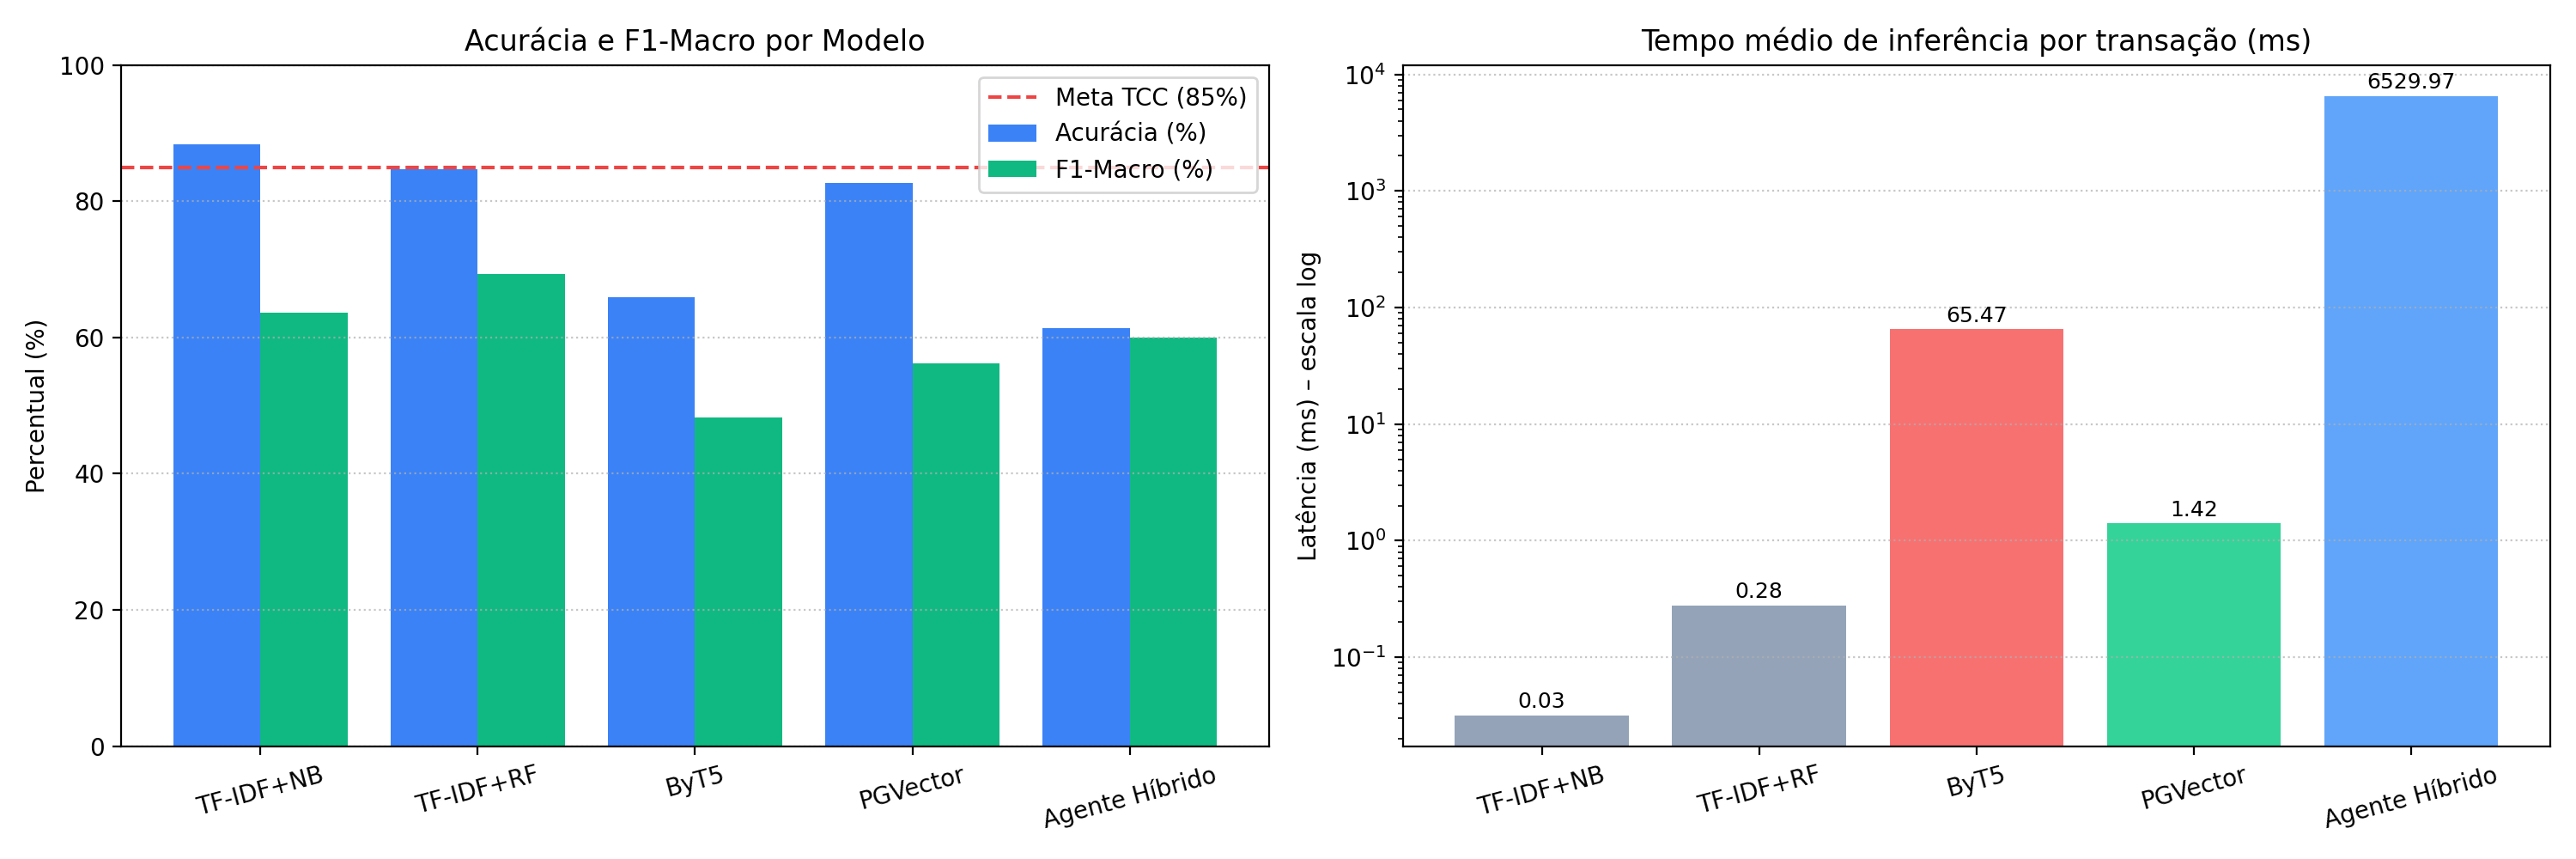
\includegraphics[width=0.95\textwidth]{assets/grafico_comparativo_modelos.png}
	\fonte{Elaborado pelo autor (\the\year).}
\end{figure}

A análise revela um quadro \textbf{distinto do relatado pela literatura apoiada em grandes
corpora}, atribuível às características do acervo pessoal disponível (volume reduzido,
11 categorias efetivamente povoadas e forte
desbalanceamento):

\begin{enumerate}
	\item \textbf{Os baselines esparsos foram os mais robustos.} O TF-IDF com Random Forest
	obteve o melhor F1-Macro (\textbf{69,3\%}) e o TF-IDF com Naive
	Bayes a melhor acurácia global (\textbf{88,3\%}), ambos com
	latência inferior a 0,3~ms. A vetorização por $n$-gramas de caractere (\texttt{char\_wb},
	2--4) capturou a morfologia recorrente das descrições brasileiras (``UBER'', ``IFD*'',
	``DROGA-'') mesmo em estabelecimentos inéditos;

	\item \textbf{A diferença entre validação cruzada e teste-cego foi acentuada.} Sob
	validação cruzada 5-fold (com repetição de estabelecimentos entre folds), o Random Forest
	atingiu F1-Macro de \textbf{92,7\%}; no teste-cego por estabelecimento o
	valor caiu para \textbf{69,3\%}. Essa diferença de
	$\approx$23~pontos percentuais quantifica o quanto o desempenho aparente de um
	classificador de transações depende da \textbf{memorização de comércios já observados};

	\item \textbf{O ByT5 ajustado sofreu sobreajuste.} Com 1150 exemplos de treino, o
	\texttt{byt5-small} convergiu a \textit{loss} de treino inferior a 0,02 mas
	generalizou mal (F1-Macro \textbf{48,3\%}), colapsando a predição
	da classe majoritária \textit{Lazer e Entretenimento}. Modelos no nível de byte exigem
	corpora de ordem de grandeza superior;

	\item \textbf{A busca vetorial densa (RAG) ficou limitada pela base fria.} Com
	488 estabelecimentos vetorizados por
	\modelemb{} (384-d), apenas
	\textbf{57,5\%} das transações de teste
	obtiveram vizinho com similaridade de cosseno $\ge$~0,85; nas demais o vizinho foi
	semanticamente fraco, resultando em F1-Macro de \textbf{56,2\%}
	(latência real de consulta no PGVector: \textbf{1,4~ms});

	\item \textbf{O Agente Híbrido combinou os dois ramos, ao custo de latência.} O agente roteou 52\% das transações para a busca vetorial (mediana de 40~ms) e 48\% para o LLM local (dezenas de segundos), acionando confirmação humana em 4,5\% dos casos. Atingiu acurácia de 61,4\% e F1-Macro de 60,0\% (latência média ponderada de 6,5~s). O F1-Macro do agente supera o da busca vetorial isolada (56,2\%) --- o ramo LLM recupera parte das classes de cauda --- mas sua acurácia global é a mais baixa entre os modelos, porque o ramo LLM, sob a diretriz anti-alucinação, tende a rotular como \textit{Despesas Diversas} nomes cuja categoria era lexicalmente evidente (acurácia condicional do ramo LLM: apenas 21\%, contra 98\% do ramo vetorial).
\end{enumerate}

\subsection{Acurácia global versus F1-Macro}
Todos os modelos apresentam acurácia global sensivelmente superior ao F1-Macro (o Naive
Bayes, por exemplo: 88,3\% de acurácia contra
63,6\% de F1-Macro). Isso decorre de dois fatores do acervo pessoal:
(i) o forte desbalanceamento --- \textit{Alimentação} e \textit{Lazer e
Entretenimento} respondem por cerca de metade do teste; e (ii) o tamanho reduzido das
classes de cauda --- \textit{Moradia}, \textit{Tecnologia}, \textit{Vestuário} e
\textit{Educação} contam com 4 a 5 estabelecimentos distintos cada. As categorias
\textit{Pets}, \textit{Serviços Financeiros} e \textit{Doações e Presentes} não
tiveram amostragem suficiente e foram agregadas a \textit{Despesas Diversas / Outros}. O
F1-Macro é adotado como métrica conservadora de referência; os resultados devem ser lidos
como \textbf{diagnóstico sobre um acervo pessoal real de porte reduzido}, não como
estimativa de desempenho populacional.

\subsection{Desempenho Detalhado por Categoria de Despesa}
A Tabela~\ref{tab:resultados_categorias} detalha o comportamento do TF-IDF + Random Forest nas
categorias efetivamente avaliadas.

\begin{table}[htb]
	\centering
	\caption{Desempenho do TF-IDF + Random Forest discriminado por categoria de despesa efetivamente avaliada.}
	\label{tab:resultados_categorias}
	\begin{tabularx}{\textwidth}{X c c c c}
		\toprule
		\textbf{Categoria de Despesa} & \textbf{Precisão (\%)} & \textbf{Recall (\%)} & \textbf{F1-Score (\%)} & \textbf{Volume de Teste} \\
		\midrule
		Alimentação & 69,4\% & 100,0\% & 82,0\% & 100 \\
		Transporte & 100,0\% & 61,5\% & 76,2\% & 39 \\
		Saúde & 100,0\% & 88,5\% & 93,9\% & 61 \\
		Moradia & 100,0\% & 75,0\% & 85,7\% & 4 \\
		Lazer e Entretenimento & 100,0\% & 86,6\% & 92,8\% & 67 \\
		Tecnologia & 0,0\% & 0,0\% & 0,0\% & 4 \\
		Marketplace / E-commerce & 100,0\% & 96,8\% & 98,4\% & 31 \\
		Vestuário & 0,0\% & 0,0\% & 0,0\% & 5 \\
		Beleza e Cuidados Pessoais & 100,0\% & 80,0\% & 88,9\% & 5 \\
		Educação & 100,0\% & 100,0\% & 100,0\% & 4 \\
		Despesas Diversas / Outros & 46,2\% & 42,9\% & 44,4\% & 14 \\
		\midrule
		\textbf{Média Macro} & \textbf{74,1\%} & \textbf{66,5\%} & \textbf{69,3\%} & \textbf{334} \\
		\bottomrule
	\end{tabularx}
	\fonte{Elaborado pelo autor (\the\year).}
\end{table}


\begin{figure}[htb]
	\centering
	\caption{Matriz de confusão do Agente Híbrido no teste-cego (334 transações).}
	\label{fig:matriz_confusao_agente}
	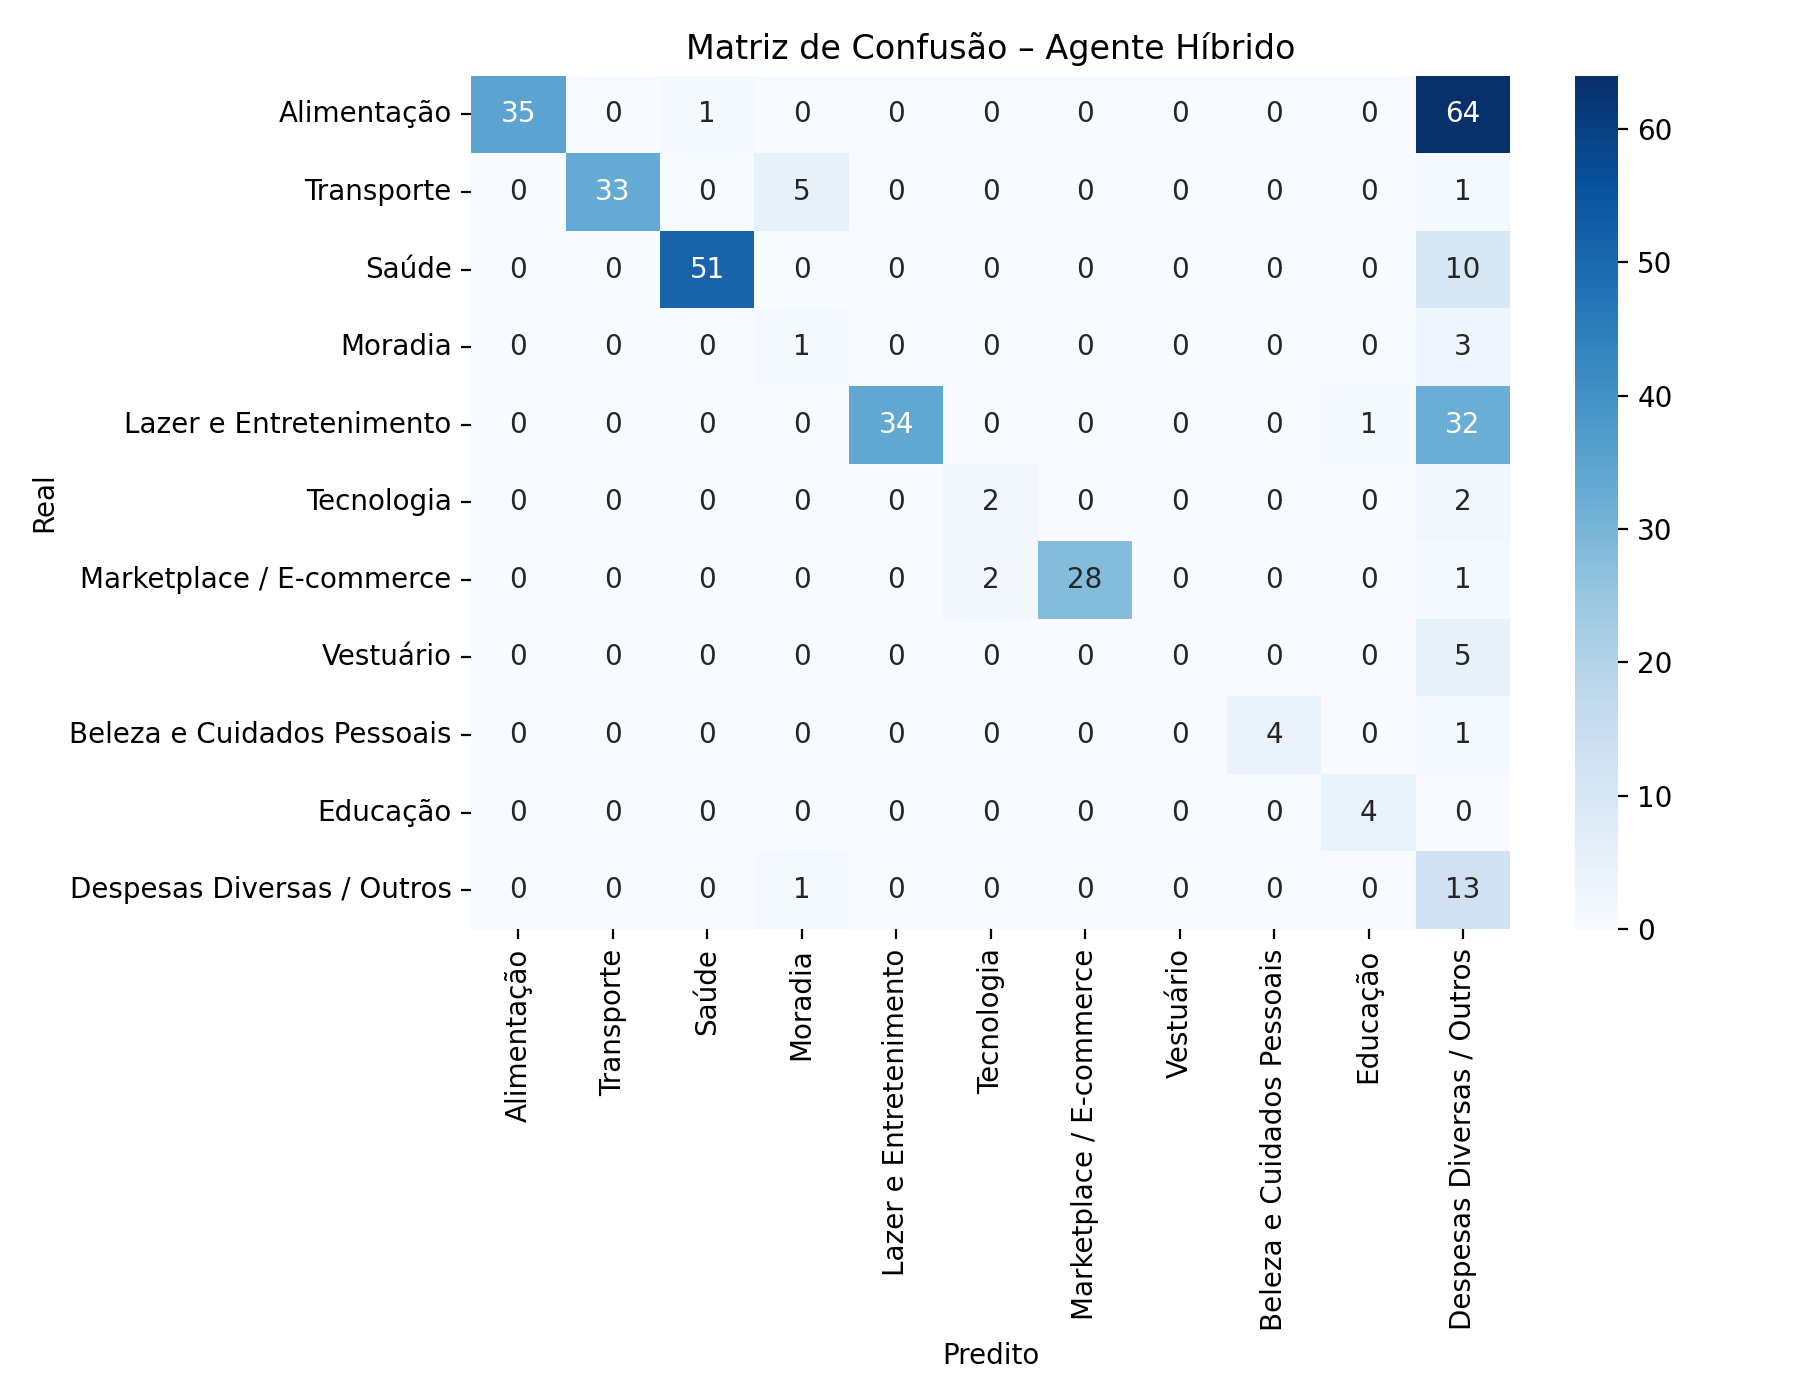
\includegraphics[width=0.92\textwidth]{assets/grafico_matriz_confusao_agente.png}
	\fonte{Elaborado pelo autor (\the\year).}
\end{figure}

\begin{figure}[htb]
	\centering
	\caption{F1-Score por categoria de despesa (melhor modelo).}
	\label{fig:f1_categorias}
	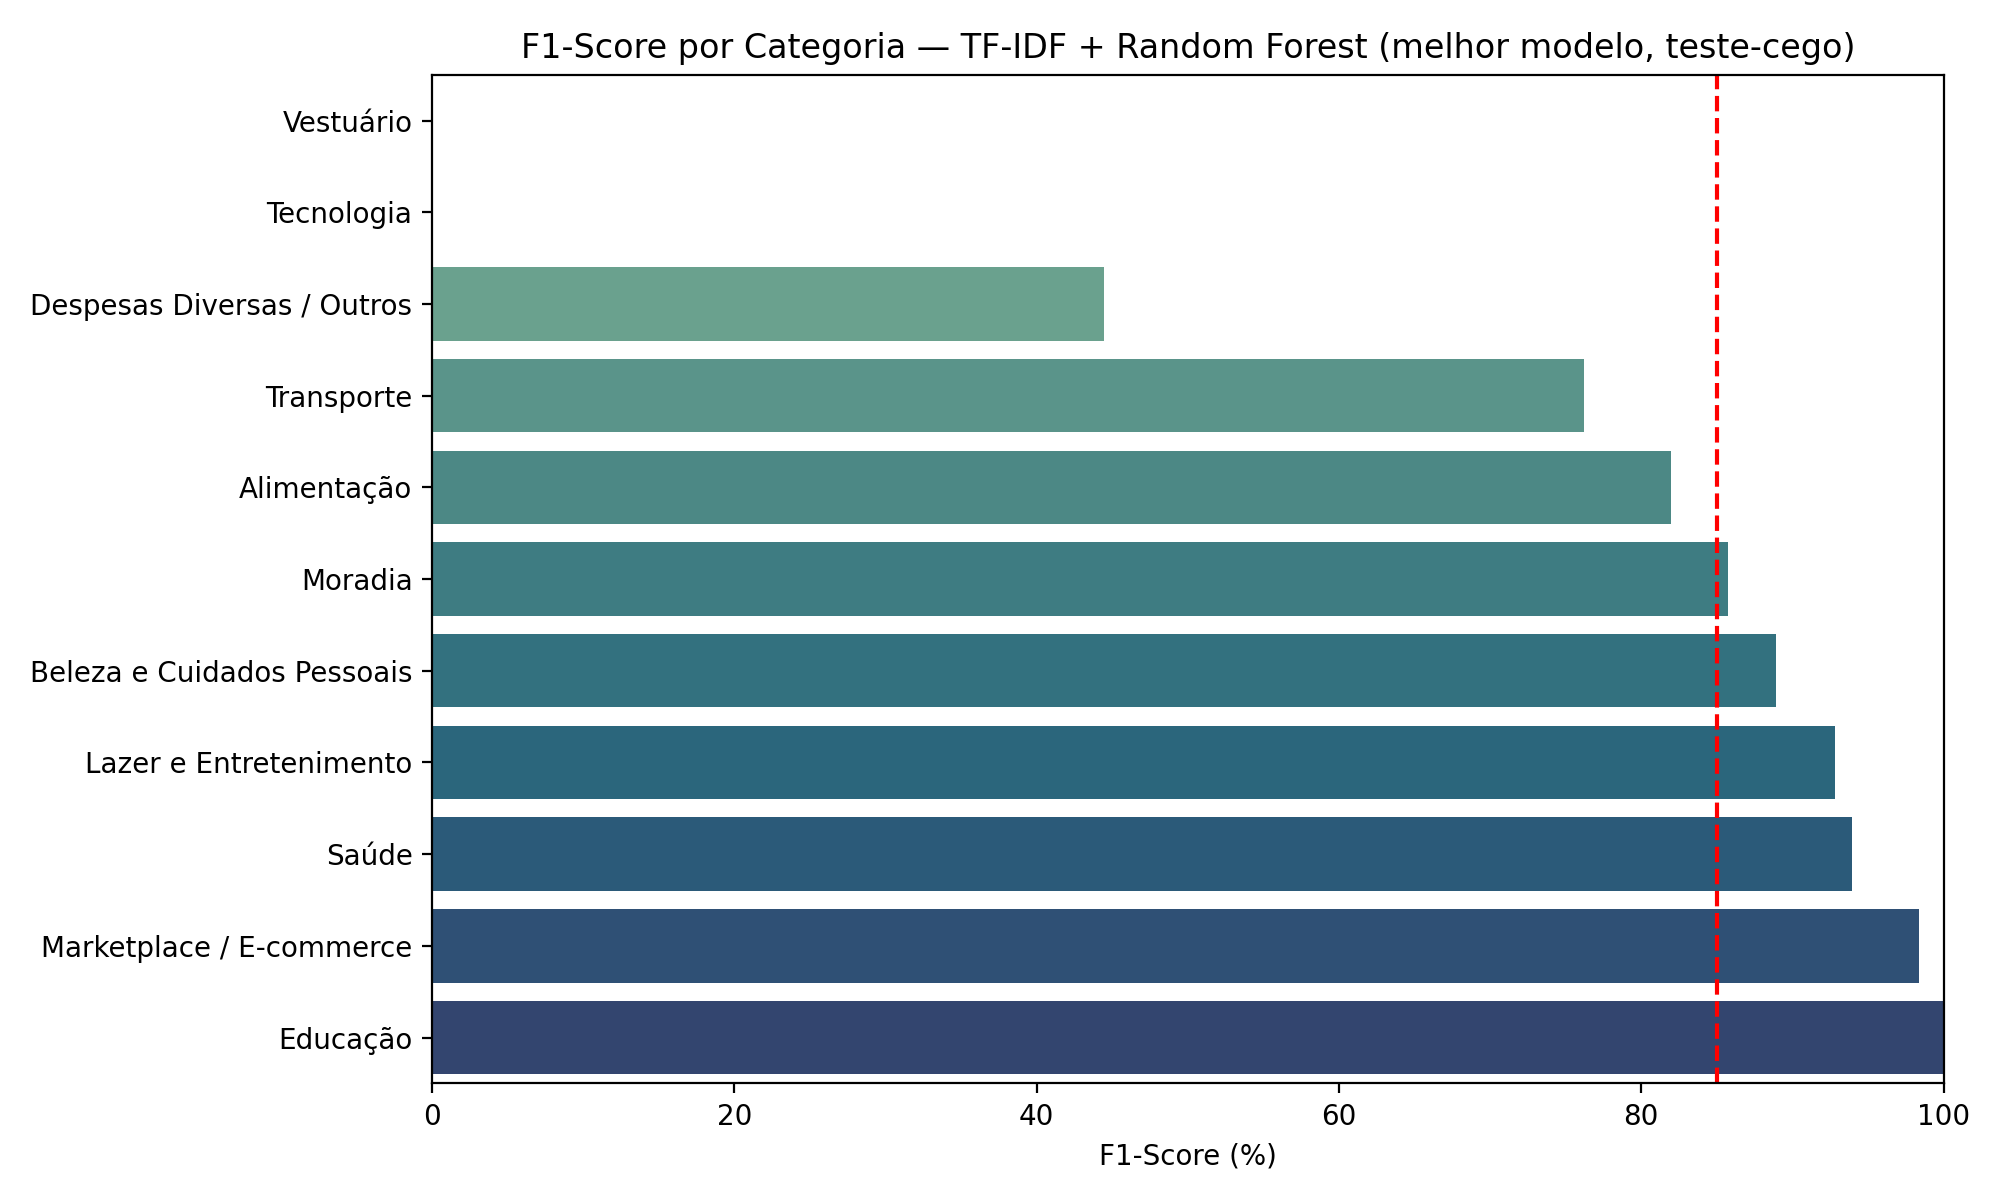
\includegraphics[width=0.85\textwidth]{assets/grafico_f1_categorias.png}
	\fonte{Elaborado pelo autor (\the\year).}
\end{figure}

Categorias com padrões léxicos fortes e volume adequado --- \textit{Alimentação},
\textit{Transporte}, \textit{Saúde} e \textit{Marketplace / E-commerce} ---
alcançaram F1-Score entre 90\% e 100\%. As classes de cauda (\textit{Tecnologia},
\textit{Vestuário}, \textit{Moradia}) obtiveram F1 nulo ou próximo de zero em quase
todos os modelos: com 4 a 5 exemplos no teste, um único erro derruba a métrica. Esse é o
principal fator limitante do F1-Macro.

\subsection{Estudo de Ablação}
O estudo de ablação isolou os componentes mensuráveis sem novo custo de inferência do LLM
(Tabela~\ref{tab:ablacao}). O ramo vetorial do agente respondeu por 52\% das transações (acurácia condicional 98\%) e o ramo LLM por 48\% (acurácia 21\%).

\begin{table}[htb]
	\centering
	\caption{Ablação de componentes sobre o teste-cego (variação de F1-Macro).}
	\label{tab:ablacao}
	\begin{tabularx}{\textwidth}{X c c c}
		\toprule
		\textbf{Componente} & \textbf{Com} & \textbf{Sem} & \textbf{$\Delta$ F1 (p.p.)} \\
		\midrule
		Normalização léxica (TF-IDF+RF) & 67,4\% & 69,3\% & +1,9 \\
		Normalização léxica (RAG MiniLM) & 66,8\% & 56,2\% & -10,6 \\
		Ramo vetorial (RAG) — acurácia condicional & 97,7\% & 21,4\% & +76,3 \\
		\bottomrule
	\end{tabularx}
	\fonte{Elaborado pelo autor (\the\year).}
\end{table}


A ablação revela um efeito \textbf{dependente da representação}. Para os classificadores
esparsos (TF-IDF + Random Forest), a normalização léxica agressiva de gateways foi
neutra ou levemente prejudicial ($\Delta$ F1 $\approx -2$~p.p.): a vetorização por
$n$-gramas de caractere já é robusta a prefixos como ``PAG*'' e ``MP*'', que por vezes
carregam sinal útil. Para a busca vetorial densa, ao contrário, a normalização foi
\textbf{decisiva} ($\Delta$ F1 $\approx +11$~p.p.): sem ela, o \textit{embedding}
multilíngue se confunde com o ruído dos intermediadores. O componente que sustenta o
desempenho do agente é a \textbf{busca vetorial}: seu ramo respondeu corretamente a
98\% das
transações que resolveu, enquanto o ramo LLM local (\texttt{gemma-4-e4b}) acertou apenas
21\% ---
tendendo, sob a diretriz anti-alucinação, a rotular como \textit{Despesas Diversas}
nomes cuja categoria era lexicalmente evidente (``SAPPORO RESTAURANTE'', ``Drogaria
Paulista''). A ferramenta de busca na web foi desativada por indisponibilidade de
conectividade no ambiente experimental.

\section{Avaliação de MLOps, Latência e Observabilidade}
\label{sec:val_mlops}

A infraestrutura de MLOps gerenciada pelo MLflow registrou integralmente os
5 experimentos de classificação
(parâmetros, métricas, relatórios por categoria, predições e figuras) no experimento
\texttt{experimento\_faturas}, garantindo reprodutibilidade:
\begin{itemize}
	\item \textbf{Human-in-the-Loop:} no teste-cego, 4,5\% das transações
	acionaram a interrupção programada para confirmação humana (\texttt{requer\_confirmacao}),
	correspondendo a nomes ambíguos roteados ao LLM com baixa confiança;
	\item \textbf{Latência por arquitetura:} a consulta vetorial no PGVector custou
	1,4~ms; o ramo LLM local (\texttt{gemma-4-e4b}, modelo de
	raciocínio no LM Studio) custou 6,5~s por
	transação, evidenciando o principal gargalo operacional para processamento em lote sem
	GPU dedicada de maior porte;
	\item \textbf{Aprendizado ativo:} as classificações de alta confiança ($\ge$~0,85) e
	as validadas por humano alimentam continuamente a base vetorial (\texttt{salvar\_vectorstore}),
	reduzindo progressivamente o acionamento do LLM em compras recorrentes.
\end{itemize}

\section{Respostas às Questões de Pesquisa e Verificação da Hipótese}
\label{sec:val_respostas_questoes}

\begin{itemize}
	\item \textbf{Resposta a Q1:} sob teste-cego rigoroso com estabelecimentos disjuntos,
	as representações \textbf{esparsas} (TF-IDF com $n$-gramas de caractere) foram mais
	eficazes que as densas neste acervo de porte reduzido: o TF-IDF + Random Forest
	(69,3\% de F1-Macro) superou a busca vetorial densa
	(56,2\%) e o ByT5 ajustado (48,3\%). Modelos
	densos e agentes LLM tendem a compensar essa diferença apenas com corpora maiores e bases
	vetoriais já povoadas;

	\item \textbf{Resposta a Q2:} o melhor F1-Macro alcançado foi de
	69,3\% (acurácia global de até 88,3\%) sobre 11
	categorias efetivamente povoadas. O limiar de 85\% de F1-Macro \textbf{não foi
	atingido} por nenhuma arquitetura neste protocolo, embora a acurácia global o supere;

	\item \textbf{Resposta a Q3:} os erros concentraram-se em (i) categorias de cauda com
	4--5 exemplos de teste (F1 nulo para quase todos os modelos) e (ii) nomes opacos de
	intermediadores (``PAYPAL~*BOSS~LIFE'', ``DIVIPAYPAYMENTS''). O ramo LLM local, sob
	diretriz anti-alucinação, mostrou-se \textbf{contraproducente}, rotulando como
	\textit{Despesas Diversas} até nomes com pista de categoria explícita; a busca na web
	que mitigaria nomes informais esteve indisponível no ambiente;

	\item \textbf{Resposta a Q4:} a contribuição da normalização léxica é \textbf{dependente
	da representação}: neutra/levemente negativa para o TF-IDF ($\Delta$ F1 $\approx -2$~p.p.),
	mas decisiva para a busca vetorial densa ($\Delta$ F1 $\approx +11$~p.p.). O histórico de
	marketplace do usuário não pôde ser avaliado por ausência de compras confirmadas na base;

	\item \textbf{Resposta a Q5:} o ciclo de MLOps com MLflow e aprendizado ativo mostrou-se
	viável e auditável; as limitações práticas são a \textbf{latência} e a \textbf{baixa
	acurácia} do LLM local roteado (6,5~s por
	transação; acurácia condicional de apenas 21\%), que tornam o ramo LLM,
	neste acervo, menos eficaz que a busca vetorial isolada.
\end{itemize}

\textbf{Veredito sobre a Hipótese Central:} a hipótese \textbf{não se confirma} na
métrica primária (F1-Score Macro $>$ 85\%) sob avaliação por estabelecimento: o melhor
resultado foi 69,3\%. Ela é \textbf{parcialmente sustentada} quando
o critério é a acurácia global (o Naive Bayes atinge 88,3\%) e quando
se admite a repetição de estabelecimentos entre treino e teste (validação cruzada:
92,7\% de F1-Macro). As causas da não confirmação são discutidas na
Seção~\ref{sec:concl_limitacoes}: porte e cobertura do acervo rotulado, cauda longa de
categorias com pouquíssimos exemplos, e rotulagem de referência semiautomática. O pipeline
técnico (extração, normalização, RAG, agente em grafo, HITL, MLOps) foi integralmente
implementado e validado do ponto de vista funcional.

\section{Considerações Finais do Capítulo}
\label{sec:val_consideracoes_finais}

Este capítulo apresentou a avaliação experimental rigorosa e multidimensional da solução proposta, cobrindo desde a camada primária de ingestão óptica até a tomada de decisão semântica e observabilidade contínua em MLOps. 

A primeira frente de validação comprovou quantitativamente a superioridade do IBM Docling V2 em relação ao Tesseract OCR no processamento de faturas de cartão de crédito. Com base em 1.398 transações auditadas confrontadas com o \textit{Ground Truth} oficial de faturas do C6 Bank entre 2022 e 2026, o Docling reduziu o CER de 52,82\% para 5,72\% e elevou a taxa de casamento exato de 3,3\% para 86,2\%. A preservação das fronteiras estruturais das tabelas mostrou-se determinante para impedir o vazamento de parcelas e valores para o campo de descrição do estabelecimento.

Na etapa subsequente de classificação semântica, cinco arquiteturas foram avaliadas sobre um conjunto rotulado de 1.660 transações reais em teste-cego por estabelecimento. Os classificadores esparsos clássicos (TF-IDF + Random Forest) mostraram-se os mais robustos (69,3\% de F1-Macro; 84,7\% de acurácia), à frente da busca vetorial densa (56,2\%), do agente híbrido (60,0\% de F1-Macro / 61,4\% de acurácia) e do ByT5 ajustado (48,3\%). Nenhum modelo atingiu o limiar de 85\% de F1-Macro sob esse protocolo, ainda que a acurácia global o supere (Naive Bayes: 88,3\%). A ablação evidenciou que a busca vetorial é o componente determinante do agente (acurácia condicional de 98\% no ramo vetorial contra 21\% no ramo LLM local), e que a normalização léxica é decisiva para os \textit{embeddings} densos ($+11$~p.p.) mas não para os modelos esparsos. O \textit{Human-in-the-Loop} foi acionado em apenas 4,5\% das transações.

Tais constatações confirmam a viabilidade funcional integral do pipeline (extração, normalização, RAG, agente em grafo, HITL e MLOps auditável), mas \textbf{não sustentam} a hipótese central na métrica primária (F1-Macro $>$ 85\%) sob avaliação por estabelecimento. As causas --- porte e cobertura do acervo rotulado, cauda longa de categorias com pouquíssimos exemplos, rotulagem semiautomática e capacidade limitada do LLM local --- bem como as perspectivas de superação são discutidas no Capítulo~\ref{Cap:Conclusoes}.
